\chapter{Advanced Software Design}


\textbf{Resorcess}
\begin{itemize}
    \item 
\end{itemize}

\section{Domain Model}
A Domain Model is a static vusual representations
of the concepts from a specific domain, i.e. from the relevant system.
If the domain is Spotify a domain element could be playlist and playSong.
%Static visual representation that illustrates meaningful concepts from a specific domain

\section{Class Diagram}
\begin{figure}[!h]
    \centering
    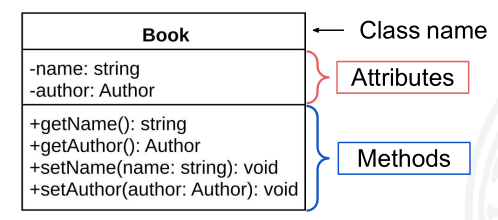
\includegraphics[width=10cm]{\imagesPath/class_structure.png}
    \caption{Class Structure. $+$ stands for public and $-$ for private. From \cite{ASD3, p.3}}
\end{figure}
\begin{figure}[!h]
    \centering
    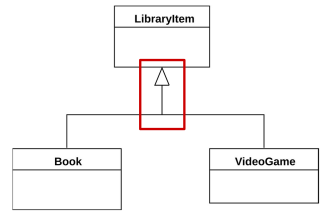
\includegraphics[width=10cm]{\imagesPath/class_relationship.png}
    \caption{Class relationship represent ``is a'', i.e. inheritance. From \cite{ASD3, p.3}}
\end{figure}
\newpage
\begin{figure}[!h]
    \centering
    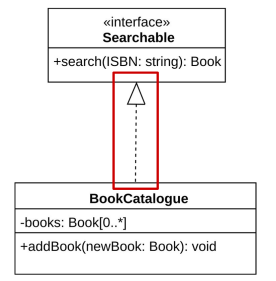
\includegraphics[width=10cm]{\imagesPath/class_interface.png}
    \caption{Class relationship represent ``is a'', i.e. inheritance. From \cite{ASD3, p.3}}
\end{figure}

Class diagram notations
\begin{itemize}
  \item Basic Association: an arrow to a class from as class
  \item Multiplicities: 1, $1..^*$, $0..^*$. Describes one-to-one, many-to-many, or one-to-many
    relationships
  \item Attribute names and visibilities: The attribute used to identify the object?
  \item Aggregation: referce to ``has a''.
  \item Composition: More strict then Aggregation.
  \item Dependency: Cannot exist unless another class exists.
  \item Qualifier (or: Key): The attribute used to identify the object.
\end{itemize}

Other
\begin{itemize}
  \item Enumeration: defines a type.
  \item Constraints: defines a constrained on a class attribute.
\end{itemize}

%\begin{itemize}
%  \item # protected
%  \item ~ package visible
%  \item + \underline{classOrStaticAttribute}:Int
%  \item + \underline{classOrStaticMethod(params)}:void
%  \item constructor: <<constructor>> ClassName(param)
%\end{itemize}


\section{GRASP}
\begin{enumerate}
    \item \textbf{Low coupling}: 
      Not dependent on too many elements.
    \item \textbf{High cohesion}: 
      No element has to many responsibilities, i.e. not to many associations.
      %measures how many responsibilities has an object.
    \item \textbf{Information expert}:
      The classes has the information to fulfil its resposibility.
      %A class that has the information to fulfil the responsibility
    \item \textbf{Pure fabrication}:
      We create classes just for the sake of increasing cohesive.
      % assign a highly cohesive set of responsibilities to a convenience class, not representing a domain concept.
    \item \textbf{Polymorphism}: 
      Classes that allowes for varing types.
      %When related alternatives or behaviors vary by type (class), assign responsibilities for this behavior - using polymorphic operations - to the types for which the behavior varies.
    \item \textbf{Indirection}:
      Create a object in between two classes, so that there are not directly coupled.
%Assign the responsibility to an intermediate object to mediate between components or services, so that they are not directly coupled. The intermediary creates and indirection between the other components.
    \item \textbf{Protected variations}:
      We design the archetecture so that changes in objects or systems doesent have a significant inpact on the rest of the system. This is for exmple done with, data encapsulation, interfaces, polymorphism, standards, virtual machines, or operating systems.
%identify points of predicted instability and create a stable responsibility around them, using:
    \item \textbf{Creator}:
      Assign responsibilities to a class to create artifacts (objects or systems).
%assign class C the responsibility to create an instance of the artifact if either:
    \item \textbf{Controller}:
\end{enumerate}


\section{Design patterns}
\subsection{Factory method}
–Define an interface for creating an object
–Subclasses decide which class to instantiate

\subsection{Abstract factory}
–Define an interface for creating families of related/dependent objects
–Concrete classes are not specified

\subsection{Builder}
–Separate the construction of complex objects from its representation
–The same process can create different representations

\subsection{Object pool}

\subsection{The Observer}